\documentclass[a4paper,12pt]{article}
\usepackage[utf8x]{inputenc}
\usepackage[skip=6pt plus1pt, indent=0.2pt]{parskip}
\usepackage{graphicx}
% \usepackage[textheight=23cm,textwidth=19cm,bottom=1.3cm,top=3cm,headsep=2.7cm]{geometry}
\usepackage[ top=5cm, left=2cm, right=2cm, headheight=4cm]{geometry}
\usepackage{enumitem}
\usepackage{listings}
\usepackage{multirow}
\usepackage{multicolumn}
\usepackage{fancyhdr}
\usepackage{tabs}
\usepackage{array}
\usepackage{url}
\usepackage{rotating}
\graphicspath{{figures/}{./images/}}
\newcommand{\eq}[1]{$#1$}
\newcommand{\head}[1]{{\bfseries #1}}
%---------------------------------------------------------------------
\newsavebox{\mytabularheader}
\newsavebox{\mytabularheadertitle}
\setlength{\extrarowheight}{0.1cm}
%------------------------------------------
\sbox{\mytabularheadertitle}{%
  \begin{minipage}{.42\textwidth}
    \begin{center}
        \bfseries \footnotesize  UNIVERSIDAD NACIONAL DE SAN AGUSTIN\\
        FACULTAD DE INGENIERÍA DE PRODUCCIÓN Y SERVICIOS\\
        ESCUELA PROFESIONAL DE INGENIERÍA DE SISTEMA\\[3mm]
    \end{center}
  \end{minipage}
}

\sbox{\mytabularheader}{%
    \begin{minipage}{\textwidth}
        \centering
        \begin{tabular}{cp{8cm}c}
            
\includegraphics[scale=0.3]{epis_logo.png} & 
            \usebox{\mytabularheadertitle} &
            
\includegraphics[scale=0.05]{abet_logo.png} \\
            % \hline
            \multicolumn{3}{c}{Formato: Guía de Práctica de Laboratorio / Talleres / Centros de Simulación}\\
             &\multicolumn{1}{c}{Aprobación:  2022/03/01 Código: GUIA-PRLE-001} &  \\
        \end{tabular}
    \end{minipage}
}
\renewcommand{\headrulewidth}{0pt}
\fancypagestyle{plain}{%
  \fancyhf{}%
  \fancyhf[ch]{\usebox{\mytabularheader}}
}
%-----------------------------------------------------------------------------------

\begin{document}
\lstset{language=Python,frame=single, firstnumber=1,basicstyle=\footnotesize,numbers=left,showspaces=false,showstringspaces=false}    
    \begin{figure}
        \centering
        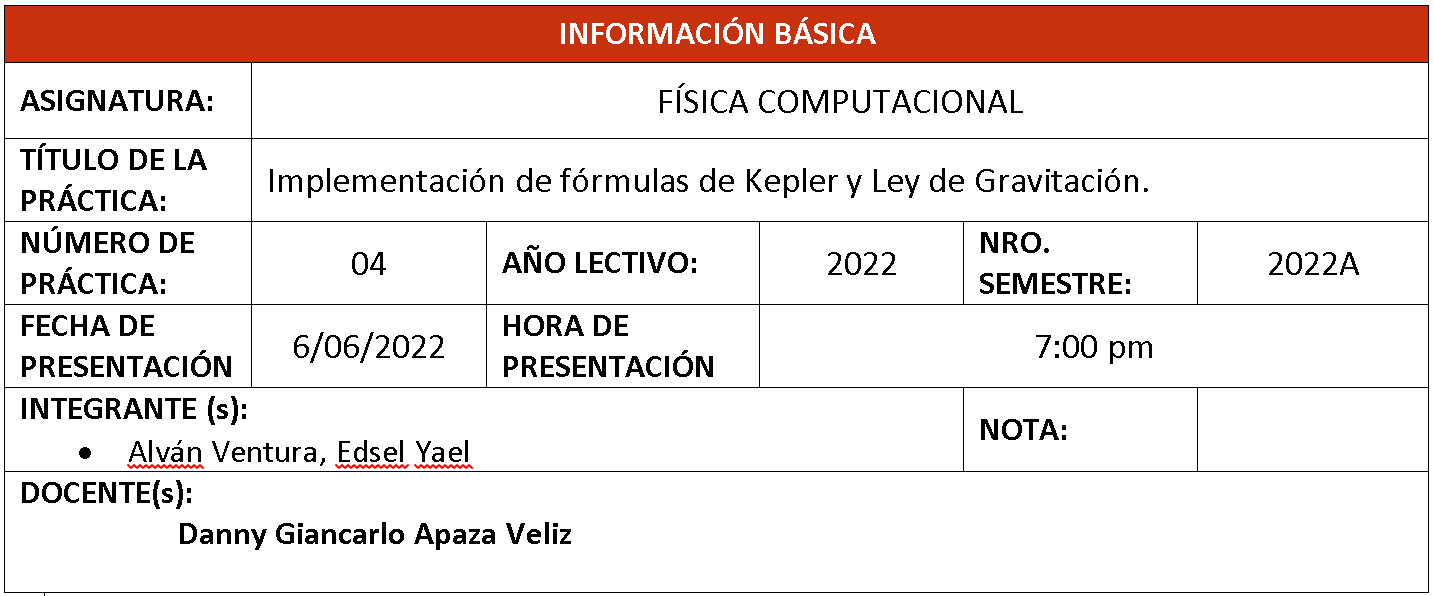
\includegraphics[scale=0.3]{tableabet}
    \end{figure}    
    
    \title{Laboratorio 04.}
    \date{\vspace{-5ex}}
    \maketitle
    \begin{center}
        Escrito por\\
        Alván Ventura, Edsel Yael\\ \texttt{ealvan@unsa.edu.pe}
        \\[3mm]
        Profesor\\Apaza Veliz, Danny Giancarlo\\ \texttt{dapazav@unsa.edu.pe}\\[3mm]
        \today
    \end{center}
    \newgeometry{top=2cm,bottom=1.4cm,right=2cm,left=2cm}
    \section{Problema 1}
        A partir de la segunda ley de movimiento de Newton 
        y la ley de gravitación universal realice un código
        que permita determinar el valor de la gravedad para 
        cualquier planeta del sistema planetario solar.
    \subsection{Análisis}
        Para obtener la gravedad en cualquier planeta del sistema 
        solar, se debe igualar la segunda ley de newton y la ley 
        de fuerza gravitacional entre dos cuerpos, pues en este
        caso la fuerza de ambas formulas son las mismas.
        A continuación se muestra la igualdad y el despeje:
        \begin{figure}[!htbp]
            \centering
            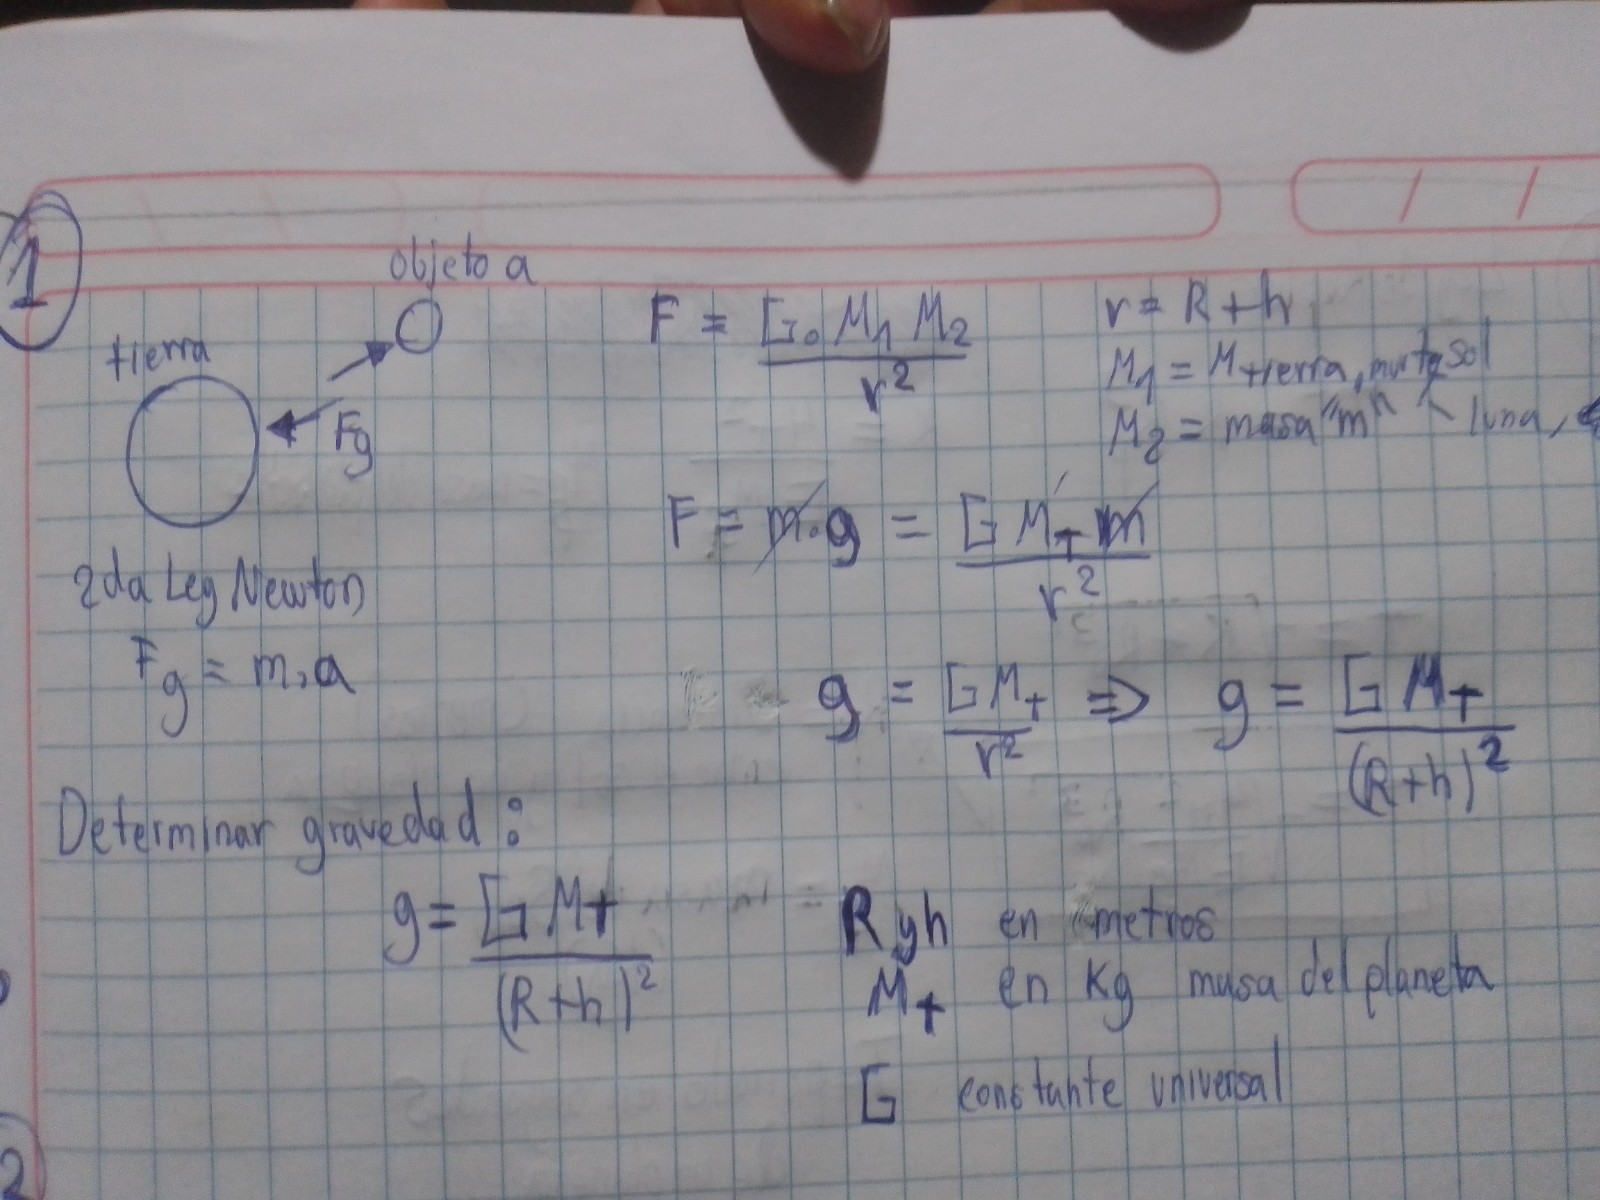
\includegraphics[scale=0.3]{ejer1fc}
        \end{figure}
    \newpage
    \subsection{Programación}
        Para la programación se obto por recolectar datos de los planetas.
        Para este caso en especifico se recolecto la masa y el radio de 
        cada planeta. Además se puso la constante universal de gravitación.
        
        Todo los datos anteriores(masa,radio) se pusieron en un 
        archivo llamado data.py, este archivo contiene un diccionario 
        en python con todos los datos(este archivo se usara continuamente
        para los siguiente ejercicios).
        \lstinputlisting[title=Archivo data.py]{data.py}

        Finalmente tambien se agrego la condición:
        \begin{lstlisting}
if h > radio:
    print("No puede ser mayor al radio del planeta")
    exit(1)#salir del programa    
        \end{lstlisting}
        A continuacion, la siguiente implementación usa el data.py para obtener los calculos con los datos de masa y radio de los planetas.
        \lstinputlisting[title=Archivo ejer1.py]{ejer1.py}

    \subsection{Resultados}
    A continuación, se muestran los calculos hechos por el algoritmo.
        \begin{table}[!htbp]
            \centering
            \begin{tabular}{cc}
                \begin{minipage}{.3\textwidth}
                    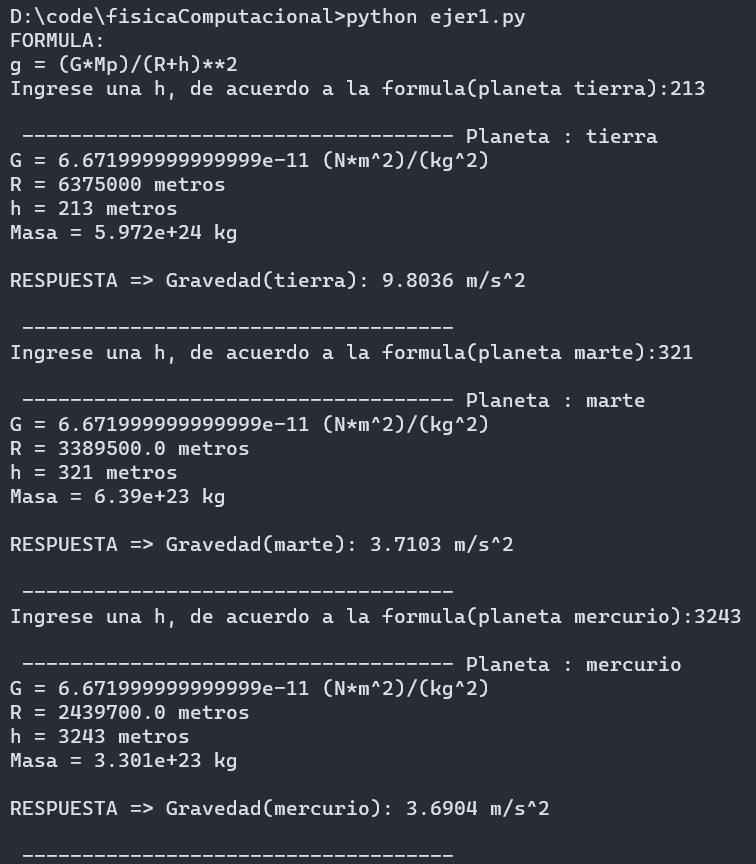
\includegraphics[width=\linewidth]{e1_1}
                \end{minipage}&\begin{minipage}{.3\textwidth}
                    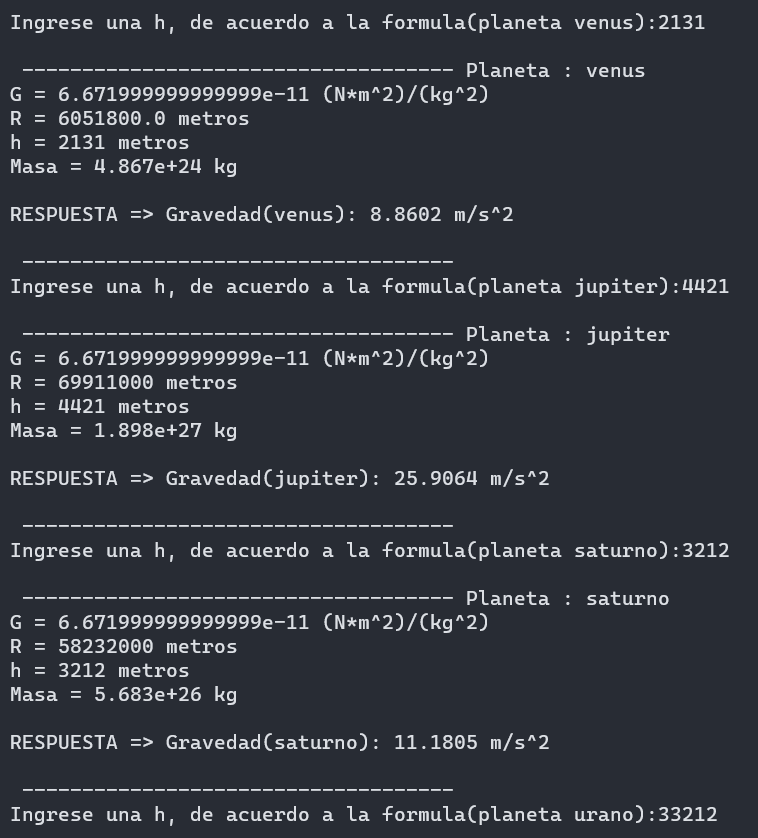
\includegraphics[width=\linewidth]{e1_2}
                \end{minipage}\\
                \begin{minipage}{.3\textwidth}
                    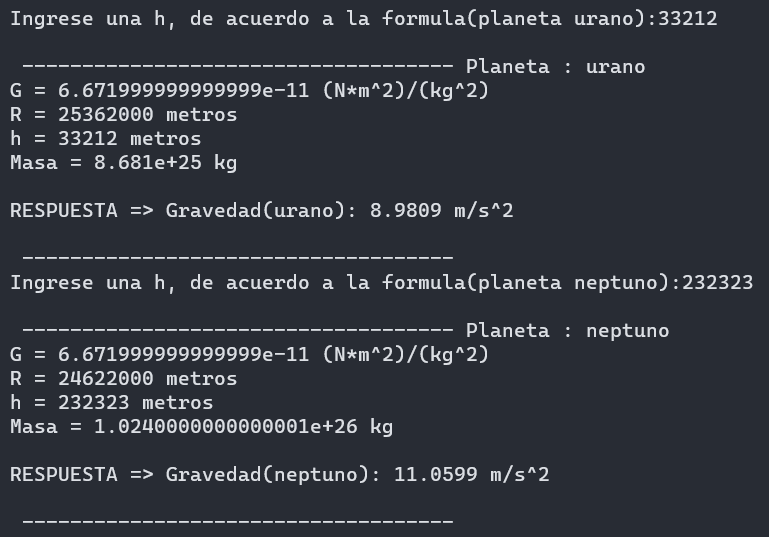
\includegraphics[width=\linewidth]{e1_3}
                \end{minipage}&\begin{minipage}{.3\textwidth}
                    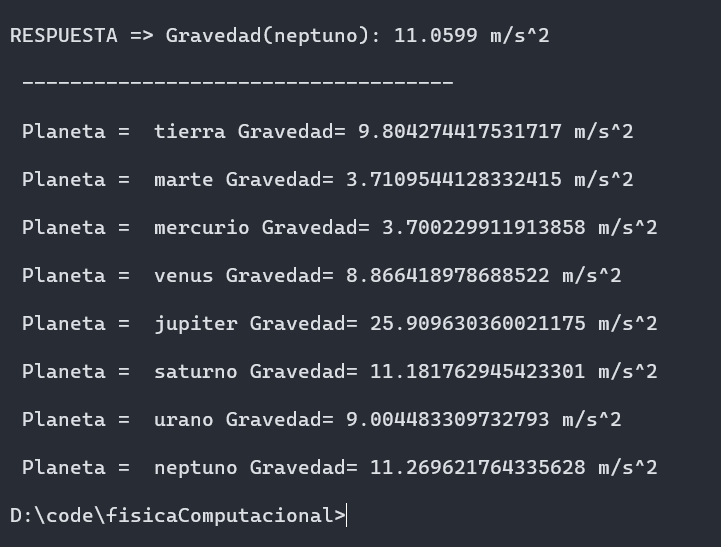
\includegraphics[width=\linewidth]{e1_4}
                \end{minipage}
            \end{tabular}
        \end{table}

        En la siguiente imagen, se muestra una comparación con datos reales:
        
        \begin{table}[!htbp]
            \centering
            \begin{tabular}{cc}
                \begin{minipage}{.3\textwidth}
                    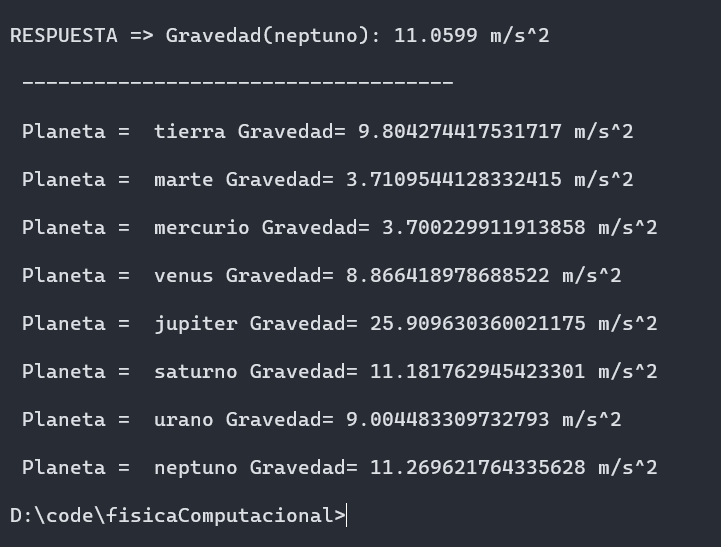
\includegraphics[width=\linewidth]{e1_4}
                \end{minipage}
                &
                \begin{minipage}{.3\textwidth}
                    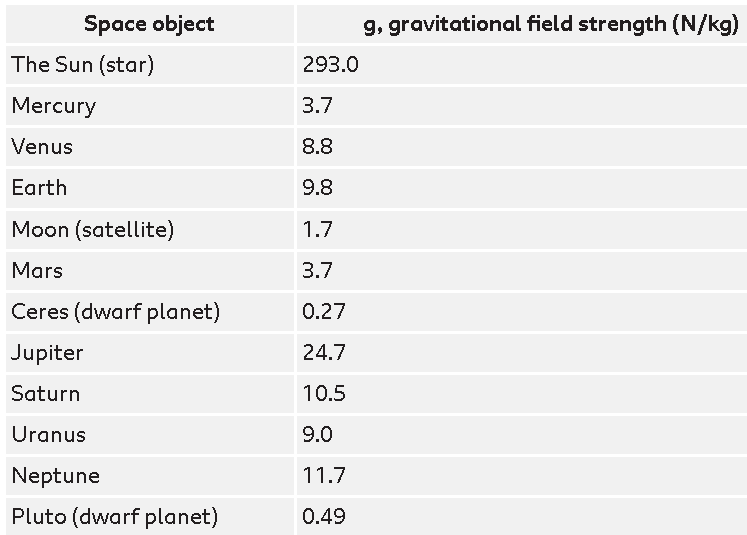
\includegraphics[width=\linewidth]{e1real}
                \end{minipage}
            \end{tabular}
        \end{table}
%---------------------------EJER 2---------------------------------------
    \section{Problema 2}
        Del problema anterior realice un código para poder 
        determinar la densidad de cualquier planeta del 
        sistema planetario solar.    
    \subsection{Análisis}
    En el siguiente analisis, se despeja la variable densidad.
    Sabiendo que:
    La densidad del planeta es:
    \begin{equation}
        \rho_p = \frac{M_p}{V_p}
    \end{equation}
    La gravedad del planeta es:
    \begin{equation}
        g_p = \frac{GM_p}{R^2}
    \end{equation}
    Y su despeje seria:
    \begin{figure}[!htbp]
        \centering
        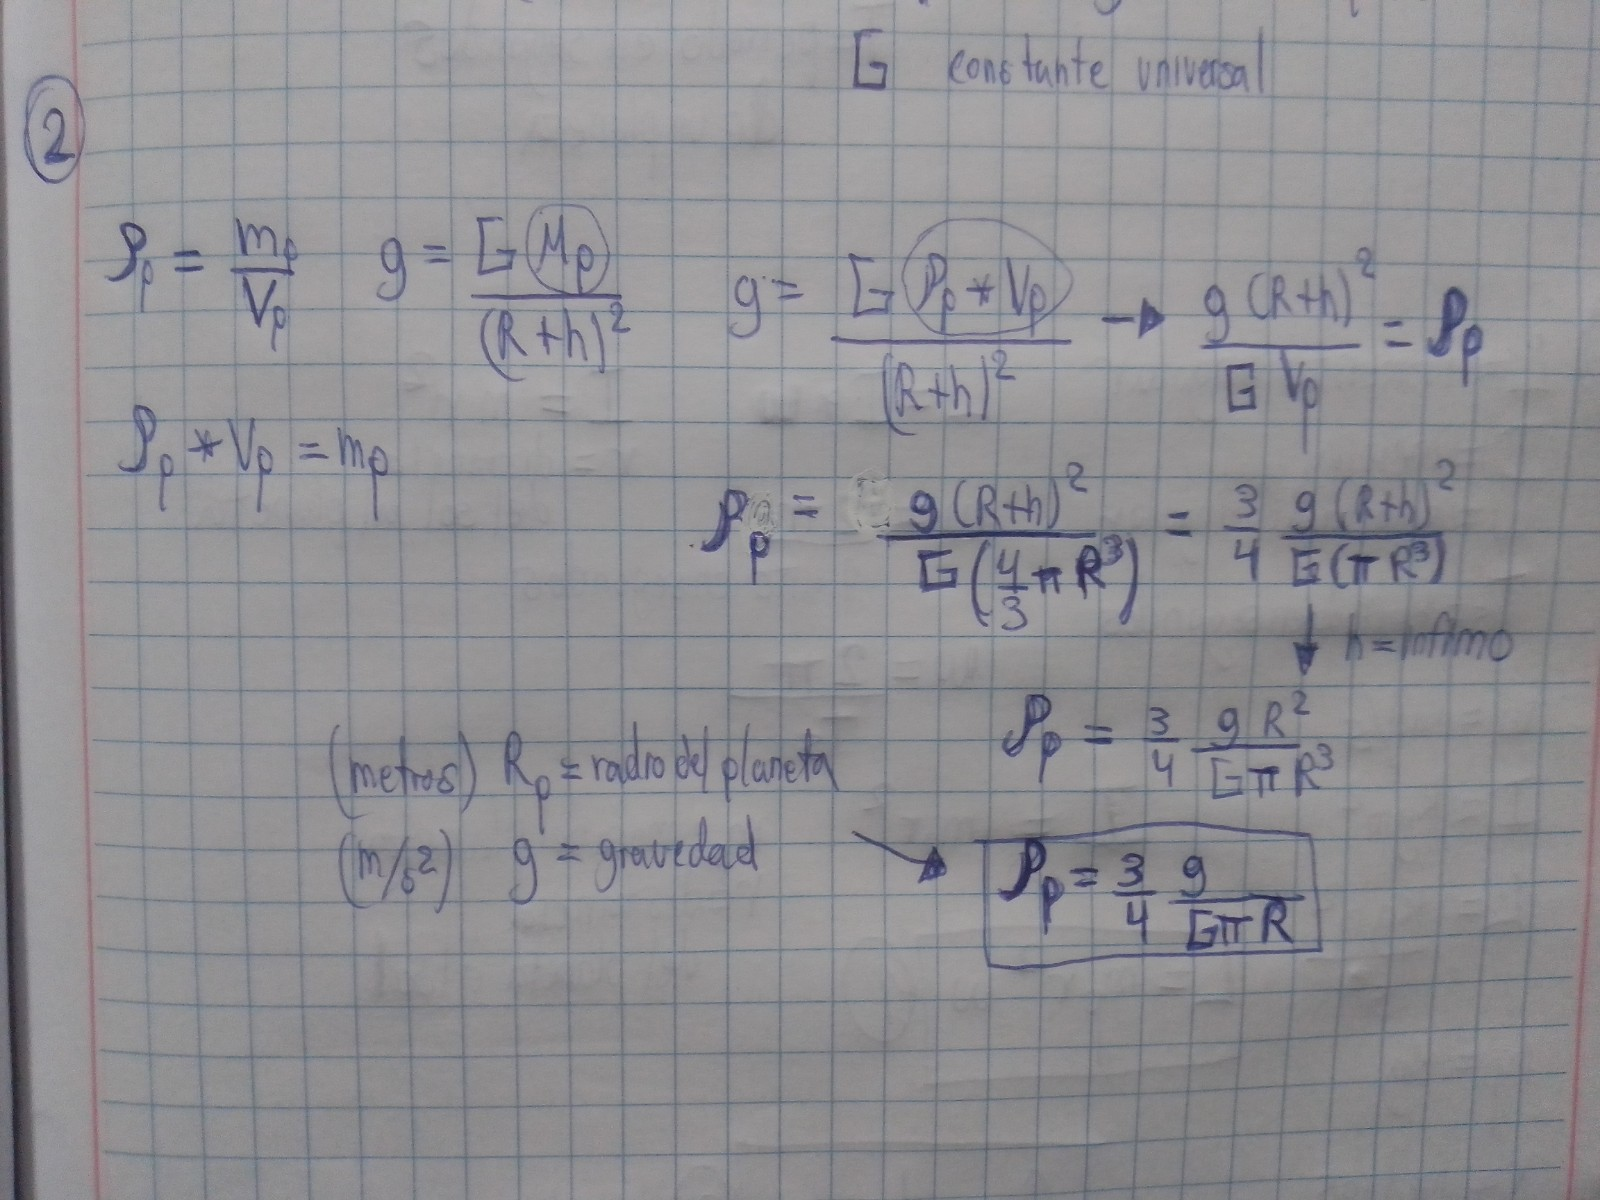
\includegraphics[scale=0.2]{ejer2fc.jpg}
    \end{figure}    

    Por lo tanto la formula seria:
    \begin{equation}
        \rho_p = (\frac{3}{4})(\frac{g_p}{G \pi R})
    \end{equation}   
    \subsection{Programación}
    En el siguiente codigo, se muestra como se implemento el codigo en el archivo ejer2.py.
    \lstinputlisting[title=Archivo ejer2.py]{ejer2.py}
    \newpage
    \subsection{Resultados}
    A continuacion se muestra los resultados obtenidos por el algoritmo:

    \begin{table}[htbp]
        \centering
        \begin{tabular}{cc}
            \begin{minipage}{.3\textwidth}
                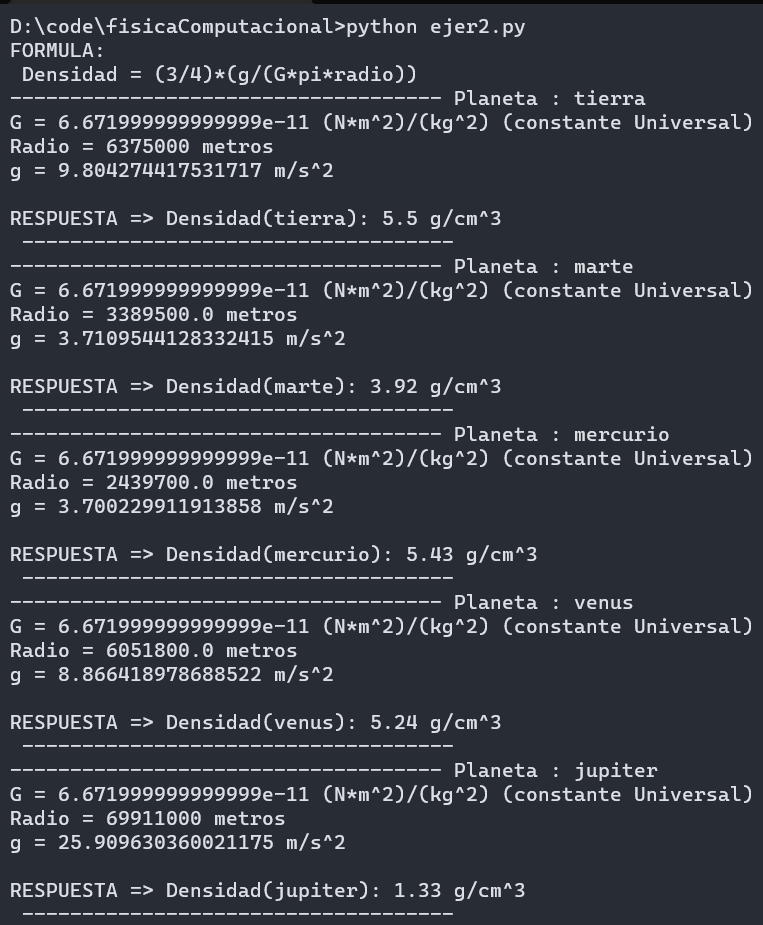
\includegraphics[width=\linewidth]{e2_1}
            \end{minipage}&
            \begin{minipage}{.3\textwidth}
                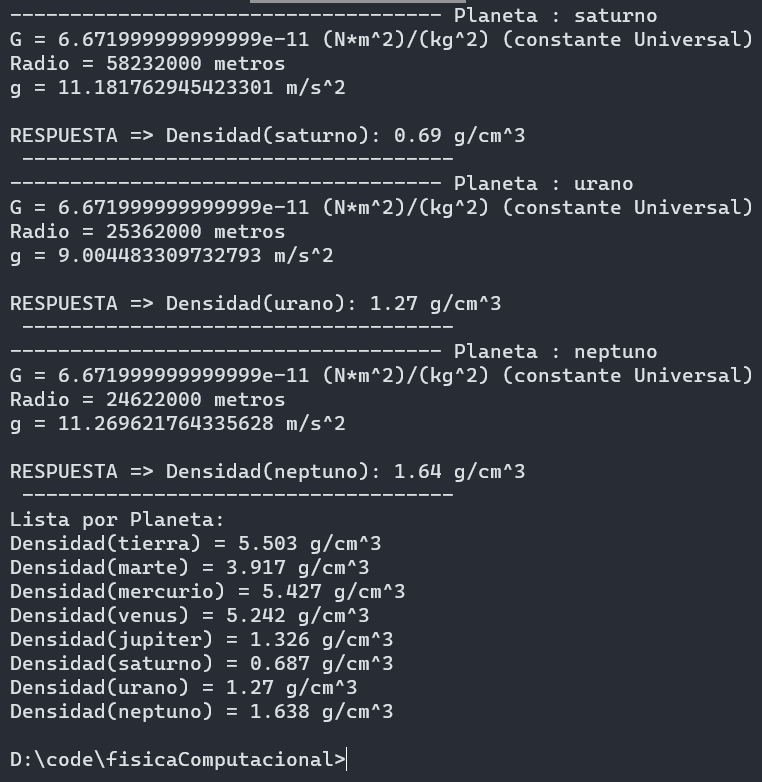
\includegraphics[width=\linewidth]{e2_2}
            \end{minipage}
        \end{tabular}
    \end{table}

    En la siguiente imagen se hace una comparacion con datos reales:
    \begin{table}[hbp]
        \centering
        \begin{tabular}{cc}
            \begin{minipage}{.3\textwidth}
                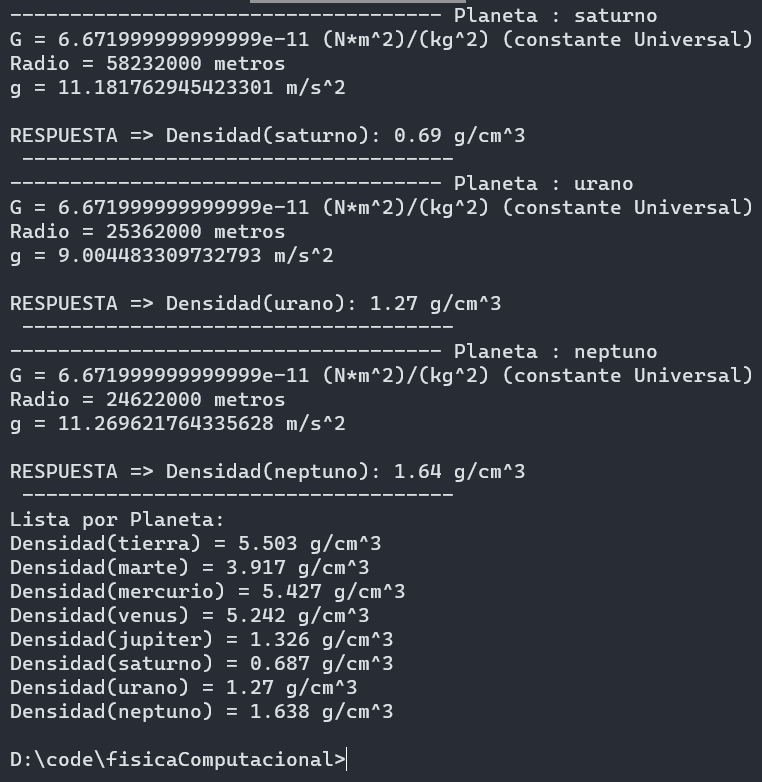
\includegraphics[width=\linewidth]{e2_2}
            \end{minipage}&
            \begin{minipage}{.3\textwidth}
                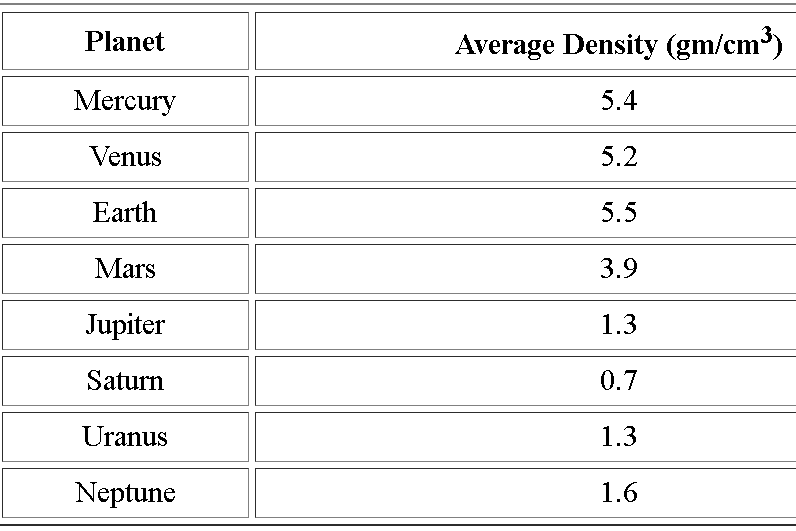
\includegraphics[width=\linewidth]{e2real}
            \end{minipage}        
        \end{tabular}
    \end{table}
    Como se puede ver los datos obtenidos son muy aproximados a los reales de las  
    densidades de cada planeta son muy aproximados.
%%------------------------------EJERCICIO 3----------------------------------
    \section{Problema 3}
    Implementar un código computacional para la 
    solución de la segunda ley de Kepler.
    \subsection{Análisis}
    La segunda ley de kepler nos dice que un planeta
    en tiempos iguales barren un area igual.

    Esto significa, un planeta cuando esta mas cerca del Sol recorre mas distancia angular en el mismo tiempo,
    mientras que el mismo planeta lejos del sol barre la misma area en el mismo tiempo, debido a que
    la distancia entre el sol y el planeta es lo suficientemente grande para barrer la misma área.

    Las siguientes ecuaciónes que se presenta se llama 
    momento de Inercia y velocidad angular:
    \begin{equation}
        I = M_p*R^2
    \end{equation}
    \begin{equation}
        w = \frac{2\pi}{1 a\tilde{n}o en segundos}
    \end{equation}
    Y el momento angular del planeta con respecto al Sol es:
    \begin{equation}
        L = Iw
    \end{equation}

    A continuacion, se ve como obtener el Area barrida por 
    un planeta con respecto al tiempo:

    \begin{figure}[htbp]
        \centering
        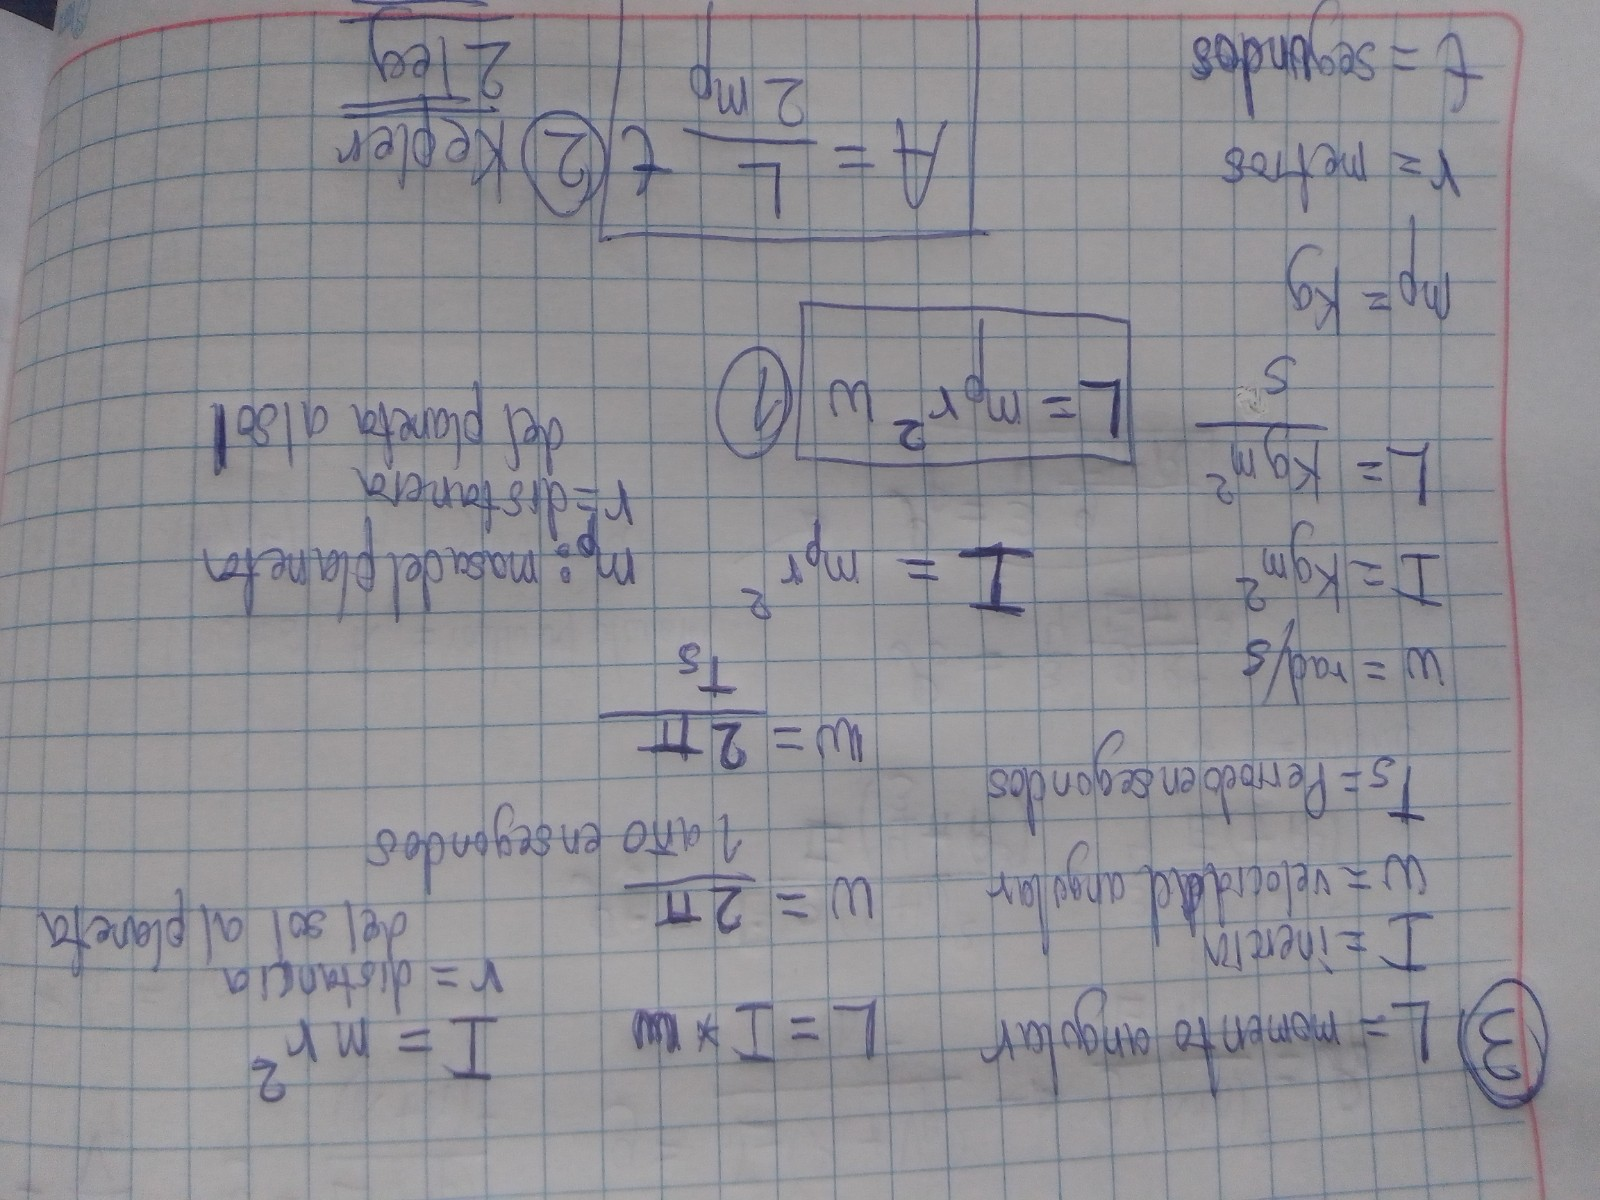
\includegraphics[scale=0.2,angle=180]{ejer3fc}
    \end{figure}
    Y la formula de la 2da ley de Kepler es:
    \begin{equation}
        A = (\frac{L_p}{2}M_p)*t
    \end{equation}
    Donde \eq{M_p} es la masa del planeta, t es el tiempo y 
    \eq{L_p} el momento angular del planeta con respecto al Sol.

    \subsection{Programación}
    En este caso se uso el archivo data.py, de este archivo usamos
    el periodo de un planeta(debemos convertirlo a segundos), 
    este nos servira para obtener "w" con mucha más exactitud.
    
    A continuación se muestra la implementación:

    \lstinputlisting[title=Archivo ejer3.py]{ejer3.py}

    \subsection{Resultados}
    Los resultados del momento angular y los de el Area recorrida se
    muestran en las siguientes imágenes:
    \begin{table}[!htbp]
        \centering
        \begin{tabular}{cc}
            \begin{minipage}{.3\textwidth}
                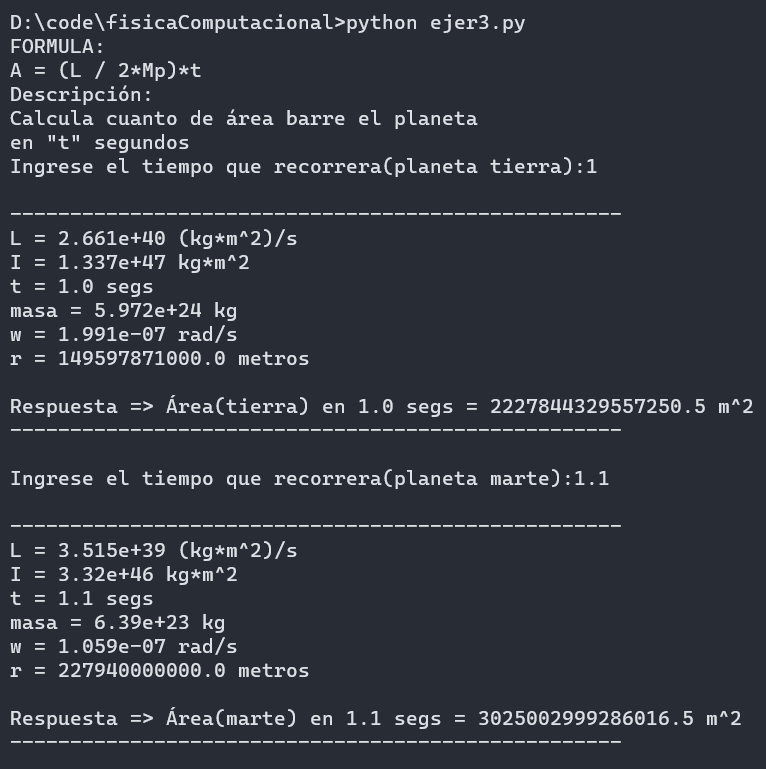
\includegraphics[width=\linewidth]{e3_1}
            \end{minipage}&\begin{minipage}{.3\textwidth}
                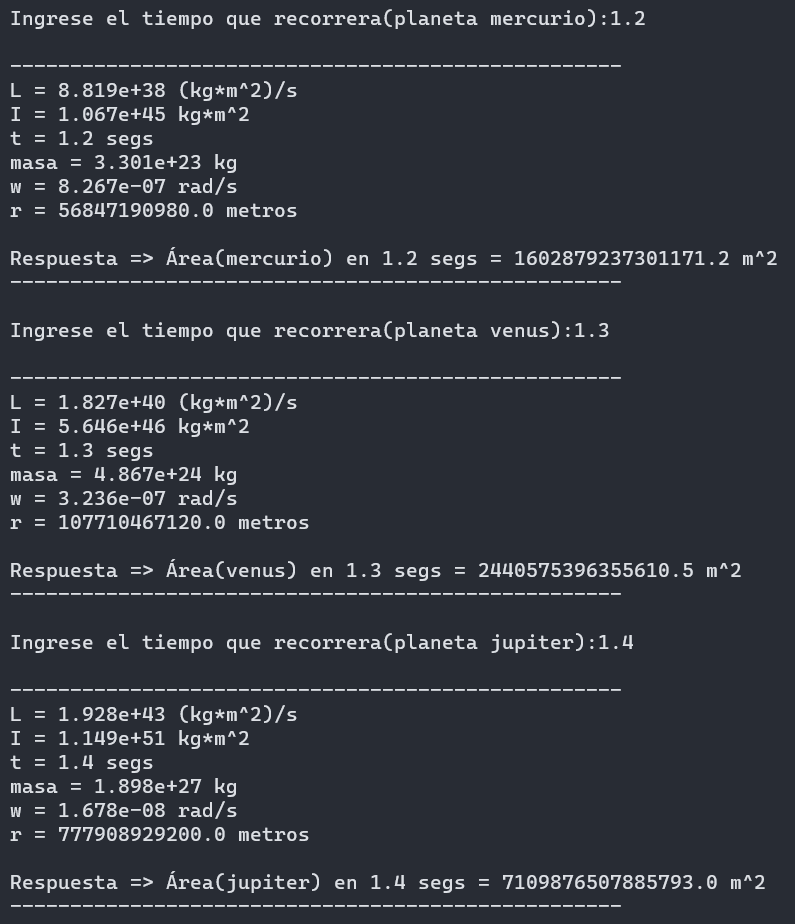
\includegraphics[width=\linewidth]{e3_2}
            \end{minipage}\\
            % \addlinespace
            \begin{minipage}{.3\textwidth}
                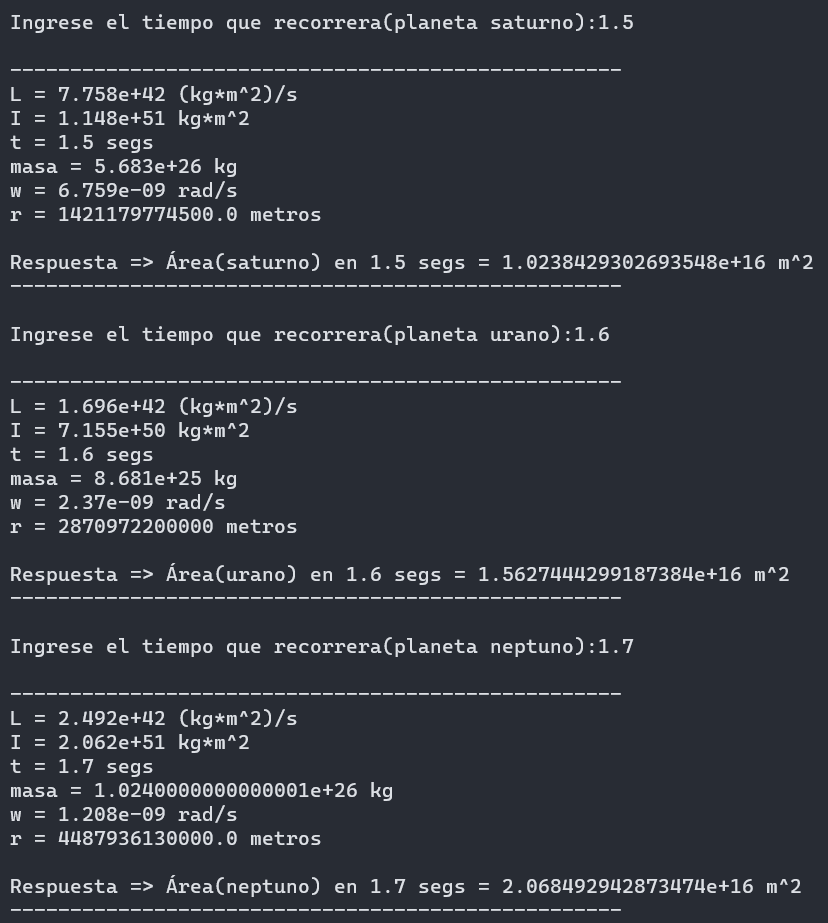
\includegraphics[width=\linewidth]{e3_3}
            \end{minipage}&\begin{minipage}{.3\textwidth}
                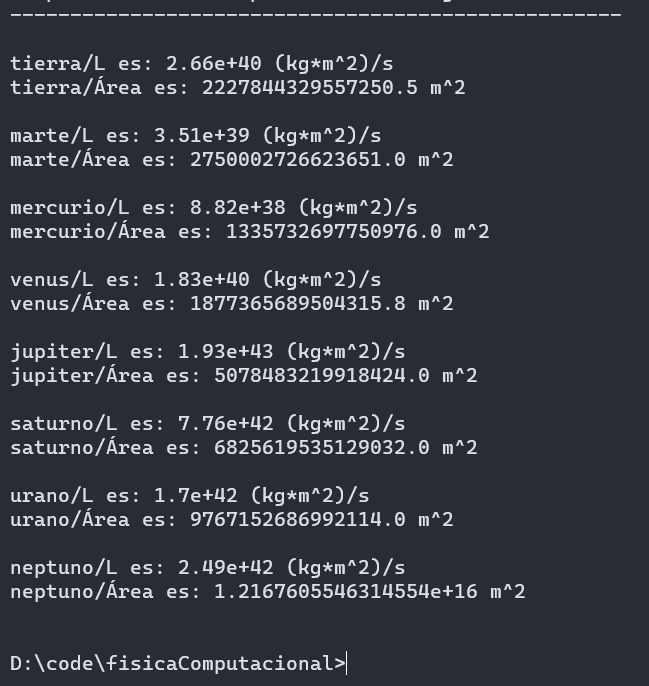
\includegraphics[width=\linewidth]{e3_4}
            \end{minipage}
        \end{tabular}
    \end{table}
    % \newpage

    A continuación se muestra una comparación entre el momento angular
    de por planeta real y el que calculamos:
    \begin{table}[!htbp]
        \centering
        \begin{tabular}{cc}
            \begin{minipage}{.3\textwidth}
                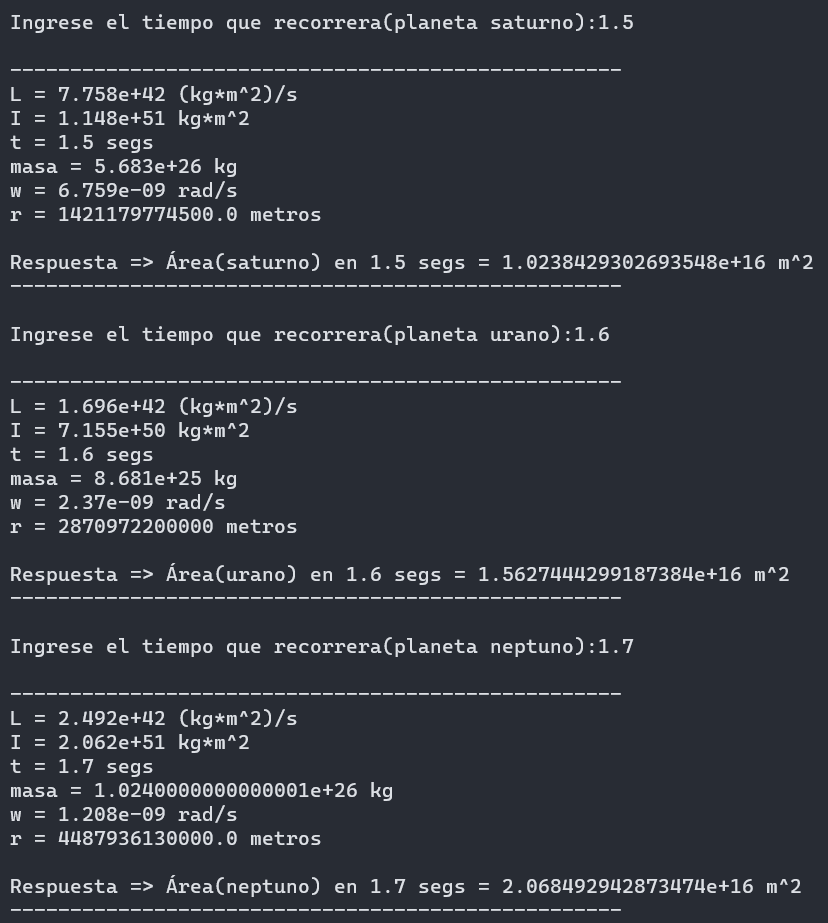
\includegraphics[width=\linewidth]{e3_3}
            \end{minipage}&\begin{minipage}{.3\textwidth}
                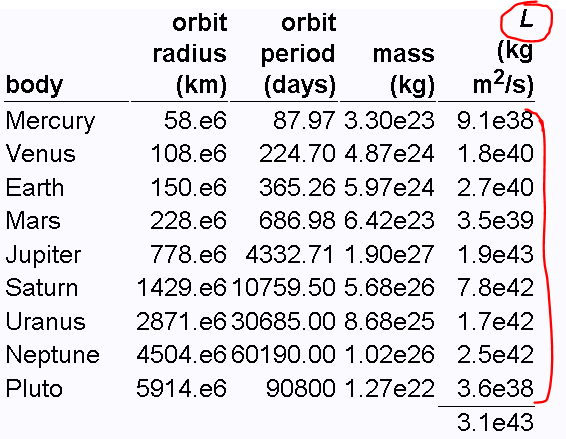
\includegraphics[width=\linewidth]{e3real}
            \end{minipage}
        \end{tabular}
    \end{table}
    Como se vio, las aproximaciones entre lo calculado y lo real, son muy aproximadas.
    
    \section{Problema 4}
    Implementar un código computacional para 
    determinar la solución de la tercera ley de 
    Kepler para cualquier planeta que describa una órbita elíptica.
    \section{Análisis}
    La 3ra ley de Kepler nos indica como obtener el periodo de un cuerpo alrededor de otro.
    En este problema calcularemos los periodos de los planetas alrededor del Sol y comprobaremos
    nuestros valores con los reales, para ver la proximidad de nuestros calculos.
    La 3ra Ley de Kepler es:
    \begin{equation}
        T^2 = KR^3
    \end{equation}    
    Tomando en cuenta que K es igual a:
    \begin{equation}
        K = \frac{4*pi^2}{GM_s}
    \end{equation}

    A continuación integrando estas dos ecuaciones, se muestra la resolución
    en la siguiente imagen:
    \begin{figure}[!ht]
        \centering
        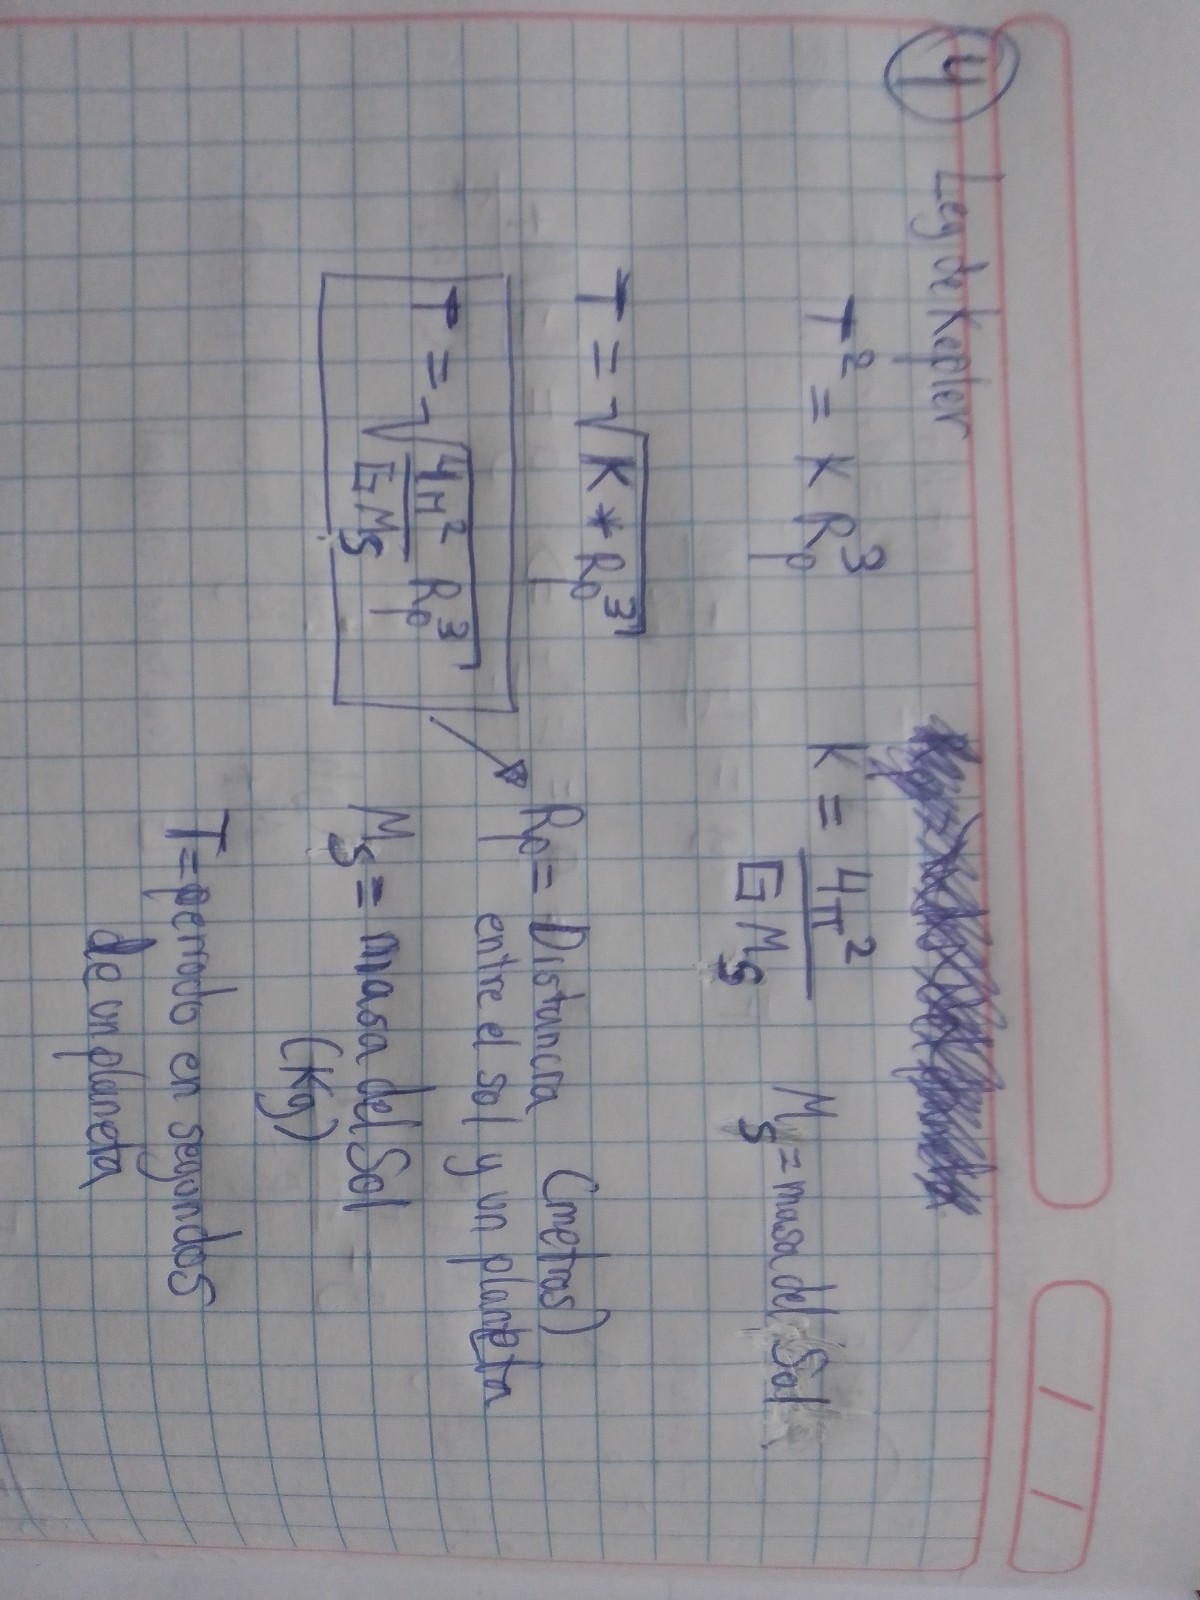
\includegraphics[scale=0.25,angle=90]{ejer4fc.jpg}        
    \end{figure}

    \section{Programación}
    Para la implementación de las formulas anteriores, se decidio tener una función llamada 
    \emph{getPeriodPlanet()}, este se encargara de obtener los datos del archivo data.py y devolver
    el periodo para cada planeta.

    A continuación se muestra el codigo de implementación:
    % \newpage
    \section{Resultados}
    Los resultados se muestran a continuación:
    \begin{table}[!htbp]
        \centering
        \begin{tabular}{cc}
            \begin{minipage}{.3\textwidth}
                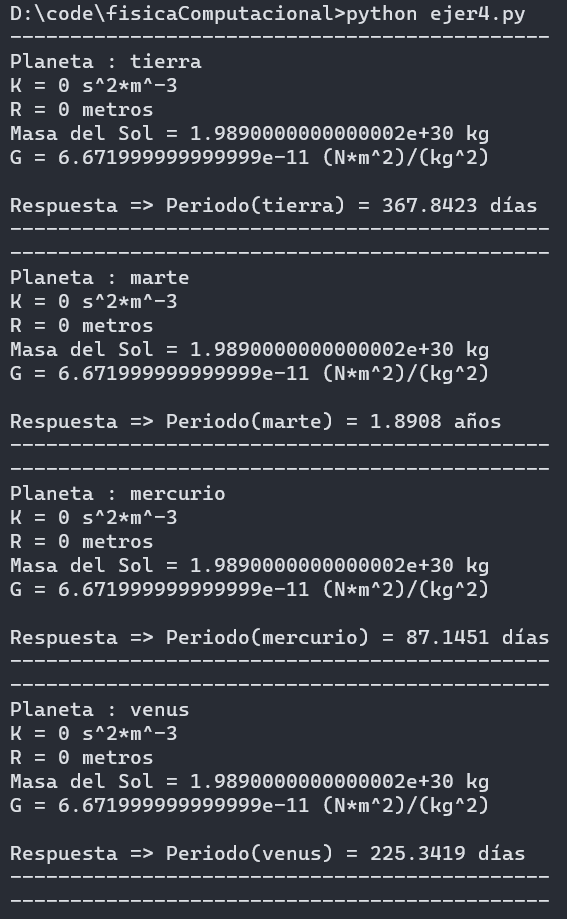
\includegraphics[width=\linewidth]{e4_1}
            \end{minipage}&\begin{minipage}{.3\textwidth}
                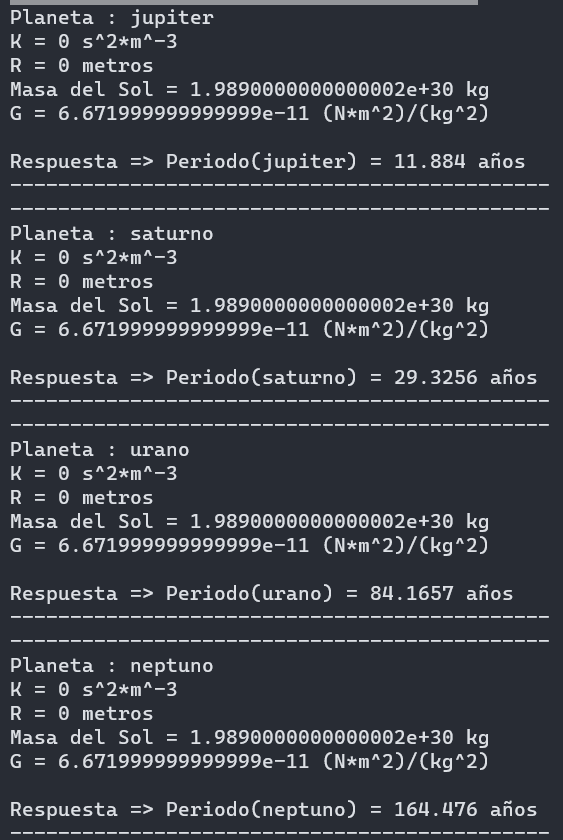
\includegraphics[width=\linewidth]{e4_2}
            \end{minipage}\\
            \multicolumn{2}{c}{
            \begin{minipage}{.3\textwidth}
                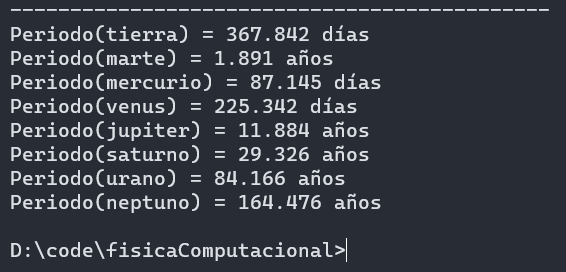
\includegraphics[width=\linewidth]{e4_3}
            \end{minipage}
            }
        \end{tabular}
    \end{table}
    % \newpage
    A continuación, se muestra una comparación entre
    los calculos y datos reales de los periodos.
    \begin{table}[!htbp]
        \centering
        \begin{tabular}{cc}
            \begin{minipage}{.3\textwidth}
                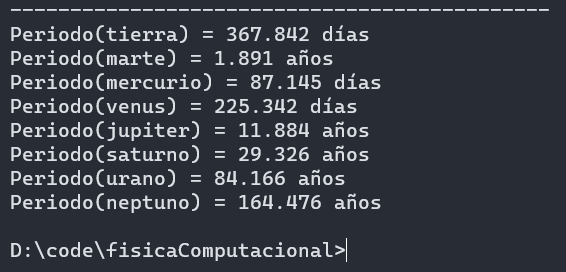
\includegraphics[width=\linewidth]{e4_3}
            \end{minipage}&\begin{minipage}{.3\textwidth}
                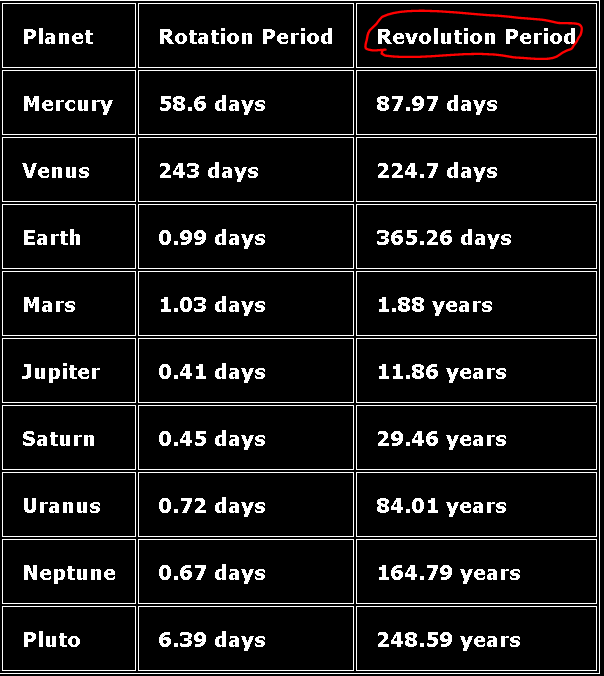
\includegraphics[width=\linewidth]{e4real}
            \end{minipage}
        \end{tabular}
    \end{table}


\end{document}
